\documentclass[12pt]{article}
\usepackage{fontspec}
\usepackage{graphicx}
\usepackage{geometry}
\usepackage{lipsum}
\usepackage[czech]{babel}
\usepackage{titling}
\usepackage{xevlna}
\usepackage{textgreek}
\usepackage{amsmath}
\usepackage[section]{placeins}
\renewcommand\maketitlehooka{\null\mbox{}\vfill}
\renewcommand\maketitlehookd{\vfill\null}
 
\setmainfont{Times New Roman}
\setlength{\parindent}{0pt} 
 
\title{MI--SPI První úloha}
\author{Tomáš Pšenička, Jan Groschaft}
\date{\today}
 
 
 % Definition of \maketitle
\makeatletter         
\def\@maketitle{
%\raggedright
\begin{center}
{\Huge \bfseries \sffamily \@title }\\[4ex] 
{\Large  \@author}\\[4ex] 
\@date\\[8ex]

\includegraphics[width = 60mm]{symbol_cvut_plna_samostatna_verze_cb.pdf}
\end{center}}
\makeatother

% \makeatletter
% \renewcommand\thesection{}
% \renewcommand\thesubsection{\@arabic\c@section.\@arabic\c@subsection}
% \makeatother


\begin{document}
 
\begin{titlingpage}
	\maketitle
\end{titlingpage}
 	
	\newpage
 
	\tableofcontents

	\newpage

 	\section{Zadání}
 		Cílem úlohy je naprogramovat konstruktivní verzi 0/1 problému batohu s užitím dynamického programování, heuristiky poměru ceny a váhy, heuristiky vybírající věc s nejvyšší cenou a algoritmem FPTAS. Výsledkem je vyhodnocení závislosti výpočetní složitosti na velikosti instance při užití různých způsobů řešení. Dále je také sledována závislost relativní chyby při zvolené přesnosti. Výpočetní složitost je měřena pomocí času potřebného pro výpočet.
 	
 		\subsection{Sady instancí}
 			Úloha řeší tři sady zadání. První sada \uv{NK} obsahuje náhodně vygenerovaná data. O druhých dvou sadách \uv{ZKC} a \uv{ZKW} ze sbírky prof. Zlomyslného nejsou známé žádné další informace. Zadané instance problému jsou v každé sadě rozděleny do souborů podle velikosti instance. Každý soubor obsahuje 500 instancí dané velikosti. Velikosti zadaných instancí jsou: 4, 10, 15, 20, 22, 25, 27, 30, 32, 35, 37, 40. S ohledem na vysokou časovou náročnost výpočtů pro velké instance obsahuje tato zpráva výsledky pro instance menší než 20 včetně.
 		
 		\subsection{Ověření výstupů}
 			Pro ověření korektnosti jsou v každé sadě příslušná řešení všech instancí pro konstrukční verzi zadaného problému. Konstrukční řešení obsahuje nejlepší dosažitelnou cenu pro danou instanci problému. Porovnáním zadané a programem zjištěné ceny lze jednoznačně určit chybovost u použitých heuristik. V souboru zadaná cena je následně pro kontrolu porovnána s výstupem implementovaného algoritmu.
 		 
 		
   		\subsection{Výpočetní platforma}
   			Implementace řešení problému je provedena v jazyce Python spouštěném na operačním systému Windows 10, po hardwarové stránce je pro výpočty využit procesor Intel Core i5--9300H.
   		
   		
   		
	\section{Popis implementovaných metod}\label{met}
		\subsection{Dynamické programování}\label{dp}
			Dynamické programování využívá ukládání počítaných mezivýsledků do dvourozměrného pole. Pro tuto metodu je použita dekompozice problému podle ceny. Na začátku je alokováno pole o velikosti $n$ (velikost instance) krát $M$ (součet cen všech předmětů v instanci). Takové pole stačí jednou projít  po prvcích a pro každý prvek rozhodnout o jeho přidaní k doposud počítaným konfiguracím a uložit výslednou váhu konfigurace na řádek, který určuje cenu této konfigurace. Poslední řádek bude obsahovat na řádcích pro všechny dostupné ceny potřebnou kapacitu. Pro získání nejlepší vhodné konfigurace stačí projít poslední sloupec od nejvyšší hodnoty a vybrat první konfiguraci, která bude splňovat požadovanou kapacitu. Složitost výpočtu je tak redukována na: \[ O(n * M)\] kde $M$ není závislé na velikosti instance. Jedná se tak o pseudopolynomiální algoritmus.
		
		
		\subsection{Heuristiky}
			První použitá heuristika vypočítá poměr ceny a váhy zadaných věcí a následně přidává předměty podle nejlepšího poměru dokud se do batohu nějaké vejdou. Takový postup vyžaduje pouze seřazení předmětů, které je možné provádět se složitostí: \[ O(n * log(n))\] Ovšem chyba tohoto postupu není obecně nijak shora omezena.
			
			Další použitá heuristika volí pouze jednu nejcennější věc, která se do batohu vejde.
			
			
		\subsection{FPTAS}\label{fptas}
			Metoda Fully Polynomial Time Approximation Scheme umožňuje provádět výpočet v polynomiálním čase s možností určení velikosti chyby. Polynomiálního času je dosaženo snížením cen předmětů. Při zadané relativní chybě $\varepsilon$ algoritmus počítá s cenou dělenou výrazem: \[K = \dfrac{\varepsilon * C_m}{n} \] Kde $C_m$ je maximální cena a $n$ je velikost instance.
			
			Výsledná relativní chyba je počítána podle vzorce:
			\[ 
			\varepsilon = 
			max\{
			\dfrac{|C(APR(I)) - C(OPT(I))|}{max\{C(OPT(I)), C(APR(I))\}} 
			\} 
			\]
Kde použité výrazy ve vzorci mají následující význam:
\begin{itemize}
\item C(S) hodnota opt. kritéria řešení S 
\item APR(I) aprox. řešení instance I 
\item OPT(I) optimální řešení instance I 
\end{itemize}			
   		
   		
   	\section{Naměřené výsledky}
   		Naměřené výsledky jsou zobrazeny v tabulkách \ref{NK_table}, \ref{ZKC_table}, \ref{ZKW_table}. Hodnoty jsou členěné podle sady ke které přísluší. Sada náhodných dat je označena písmenem \uv{NK} a sady prof. Zlomyslného \uv{ZKC} a \uv{ZKW}. Pro výpočet jsou použity postupy popsané v sekci \ref{met}. Tabulky obsahují časy běhu pro různé algoritmy v sekundách naměřené pomocí nástroje \textit{cProfile}.
   		
   		Hodnoty z tabulek jsou zobrazeny na grafech \ref{ZKC_graph} a \ref{ZKW_graph}. Z grafu je patrná velká časová náročnost přesného dynamického programování oproti ostatním aproximativním způsobům řešení.
   		
   		Naměřené maximální chyby jsou zobrazeny v tabulkách \ref{NK_error_table}, \ref{ZKC_error_table} a \ref{ZKW_error_table}. Chyba je pro všechny aproximativní algoritmy vypočítána podle vzorečku ze sekce \ref{fptas}. Dynamické programování dává přesné výsledky, proto pro něj nedává smysl určovat chybu. Chyba s hodnotou $1.0$ vznikla v případě, kdy FPTAS vrátil konfiguraci samých nul i když bylo možné do batohu nějaký předmět vložit.
   		
   		
\begin{table}[h!]
\centering
\begin{tabular}{ | c | | c | c | c | c | }\hline
Velikost instance & 4 & 10 & 15 & 20 \\ \hline \hline
Dynamické programování & 8.569 & 86.187 & 181.436 & 539.184  \\ \hline
FPTAS ε=0.1 & 0.111 & 2.5 & 11.208 & 38.303  \\ \hline
FPTAS ε=0.2 & 0.074 & 1.258 & 5.264 & 18.095  \\ \hline
FPTAS ε=0.3 & 0.06 & 0.835 & 4.615 & 10.849  \\ \hline
FPTAS ε=0.4 & 0.05 & 0.633 & 2.973 & 9.137  \\ \hline
FPTAS ε=0.5 & 0.046 & 0.523 & 2.184 & 7.402  \\ \hline
Heuristika poměru cena váha & 0.027 & 0.038 & 0.045 & 0.055  \\ \hline
Heuristika jeden předmět & 0.025 & 0.036 & 0.039 & 0.05  \\ \hline
\end{tabular}
\caption{Průměrné naměřené časy v sekundách sady NK.}
\label{NK_table}
\end{table}

\begin{table}[h!]
\centering
\begin{tabular}{ | c | | c | c | c | c | }\hline
Velikost instance & 4 & 10 & 15 & 20 \\ \hline \hline
FPTAS ε=0.1 & 0.014358 & 0.002134 & 0.003003 & 1.0  \\ \hline
FPTAS ε=0.2 & 1.0 & 0.078431 & 0.005986 & 1.0  \\ \hline
FPTAS ε=0.3 & 1.0 & 0.078431 & 0.005986 & 1.0  \\ \hline
FPTAS ε=0.4 & 1.0 & 0.078431 & 0.00815 & 1.0  \\ \hline
FPTAS ε=0.5 & 1.0 & 0.078431 & 0.00815 & 1.0  \\ \hline
Heuristika poměru cena váha & 0.359189 & 0.531453 & 0.236835 & 0.430054  \\ \hline
Heuristika jeden předmět & 0.663519 & 0.8689 & 0.906724 & 0.925672  \\ \hline
\end{tabular}
\caption{Naměřená maximální chyba podle použitého algoritmu a velikosti instance, sada  NK.}
\label{NK_error_table}
\end{table}

\begin{table}[h!]
\centering
\begin{tabular}{ | c | | c | c | c | c | }\hline
Velikost instance & 4 & 10 & 15 & 20 \\ \hline \hline
Dynamické programování & 9.347 & 89.662 & 192.831 & 588.504  \\ \hline
FPTAS ε=0.1 & 0.144 & 2.752 & 11.358 & 40.698  \\ \hline
FPTAS ε=0.2 & 0.087 & 1.358 & 5.433 & 18.739  \\ \hline
FPTAS ε=0.3 & 0.064 & 1.21 & 4.712 & 13.018  \\ \hline
FPTAS ε=0.4 & 0.054 & 0.903 & 2.689 & 8.624  \\ \hline
FPTAS ε=0.5 & 0.05 & 0.592 & 2.092 & 6.889  \\ \hline
Heuristika poměru cena váha & 0.027 & 0.038 & 0.047 & 0.075  \\ \hline
Heuristika jeden předmět & 0.025 & 0.036 & 0.042 & 0.054  \\ \hline
\end{tabular}
\caption{Průměrné naměřené časy v sekundách sady ZKC.}
\label{ZKC_table}
\end{table}

\begin{table}[h!]
\centering
\begin{tabular}{ | c | | c | c | c | c | }\hline
Velikost instance & 4 & 10 & 15 & 20 \\ \hline \hline
FPTAS ε=0.1 & 0.017082 & 0.004709 & 0.002029 & 0.001215  \\ \hline
FPTAS ε=0.2 & 0.040284 & 0.011128 & 0.004442 & 0.002303  \\ \hline
FPTAS ε=0.3 & 0.078697 & 0.013054 & 0.005952 & 0.003454  \\ \hline
FPTAS ε=0.4 & 0.13494 & 0.018066 & 0.007311 & 0.004749  \\ \hline
FPTAS ε=0.5 & 0.207725 & 0.037775 & 0.008352 & 0.007452  \\ \hline
Heuristika poměru cena váha & 0.490298 & 0.249584 & 0.154858 & 0.111739  \\ \hline
Heuristika jeden předmět & 0.62952 & 0.803984 & 0.862146 & 0.891126  \\ \hline
\end{tabular}
\caption{Naměřená maximální chyba podle použitého algoritmu a velikosti instance, sada  ZKC.}
\label{ZKC_error_table}
\end{table}

\begin{table}[h!]
\centering
\begin{tabular}{ | c | | c | c | c | c | }\hline
Velikost instance & 4 & 10 & 15 & 20 \\ \hline \hline
Dynamické programování & 42.055 & 72.809 & 65.279 & 96.475  \\ \hline
FPTAS ε=0.1 & 0.225 & 0.851 & 1.913 & 3.505  \\ \hline
FPTAS ε=0.2 & 0.173 & 0.425 & 0.898 & 1.566  \\ \hline
FPTAS ε=0.3 & 0.149 & 0.352 & 0.692 & 1.076  \\ \hline
FPTAS ε=0.4 & 0.133 & 0.306 & 0.471 & 0.685  \\ \hline
FPTAS ε=0.5 & 0.159 & 0.175 & 0.398 & 0.565  \\ \hline
Heuristika poměru cena váha & 0.084 & 0.016 & 0.006 & 0.003  \\ \hline
Heuristika jeden předmět & 0.084 & 0.014 & 0.005 & 0.002  \\ \hline
\end{tabular}
\caption{Průměrné naměřené časy v sekundách sady ZKW.}
\label{ZKW_table}
\end{table}

\begin{table}[h!]
\centering
\begin{tabular}{ | c | | c | c | c | c | }\hline
Velikost instance & 4 & 10 & 15 & 20 \\ \hline \hline
FPTAS ε=0.1 & 0.033204 & 0.01622 & 0.009777 & 0.009248  \\ \hline
FPTAS ε=0.2 & 0.045822 & 0.051179 & 0.036217 & 0.017655  \\ \hline
FPTAS ε=0.3 & 0.092338 & 0.07656 & 0.053289 & 0.017655  \\ \hline
FPTAS ε=0.4 & 0.14166 & 0.07656 & 0.064089 & 0.026297  \\ \hline
FPTAS ε=0.5 & 0.258182 & 0.118424 & 0.081173 & 0.079371  \\ \hline
Heuristika poměru cena váha & 0.992908 & 0.987585 & 0.9375 & 0.760458  \\ \hline
Heuristika jeden předmět & 0.143221 & 0.213391 & 0.219789 & 0.132229  \\ \hline
\end{tabular}
\caption{Naměřená maximální chyba podle použitého algoritmu a velikosti instance, sada  ZKW.}
\label{ZKW_error_table}
\end{table}

\begin{figure}[!htb]
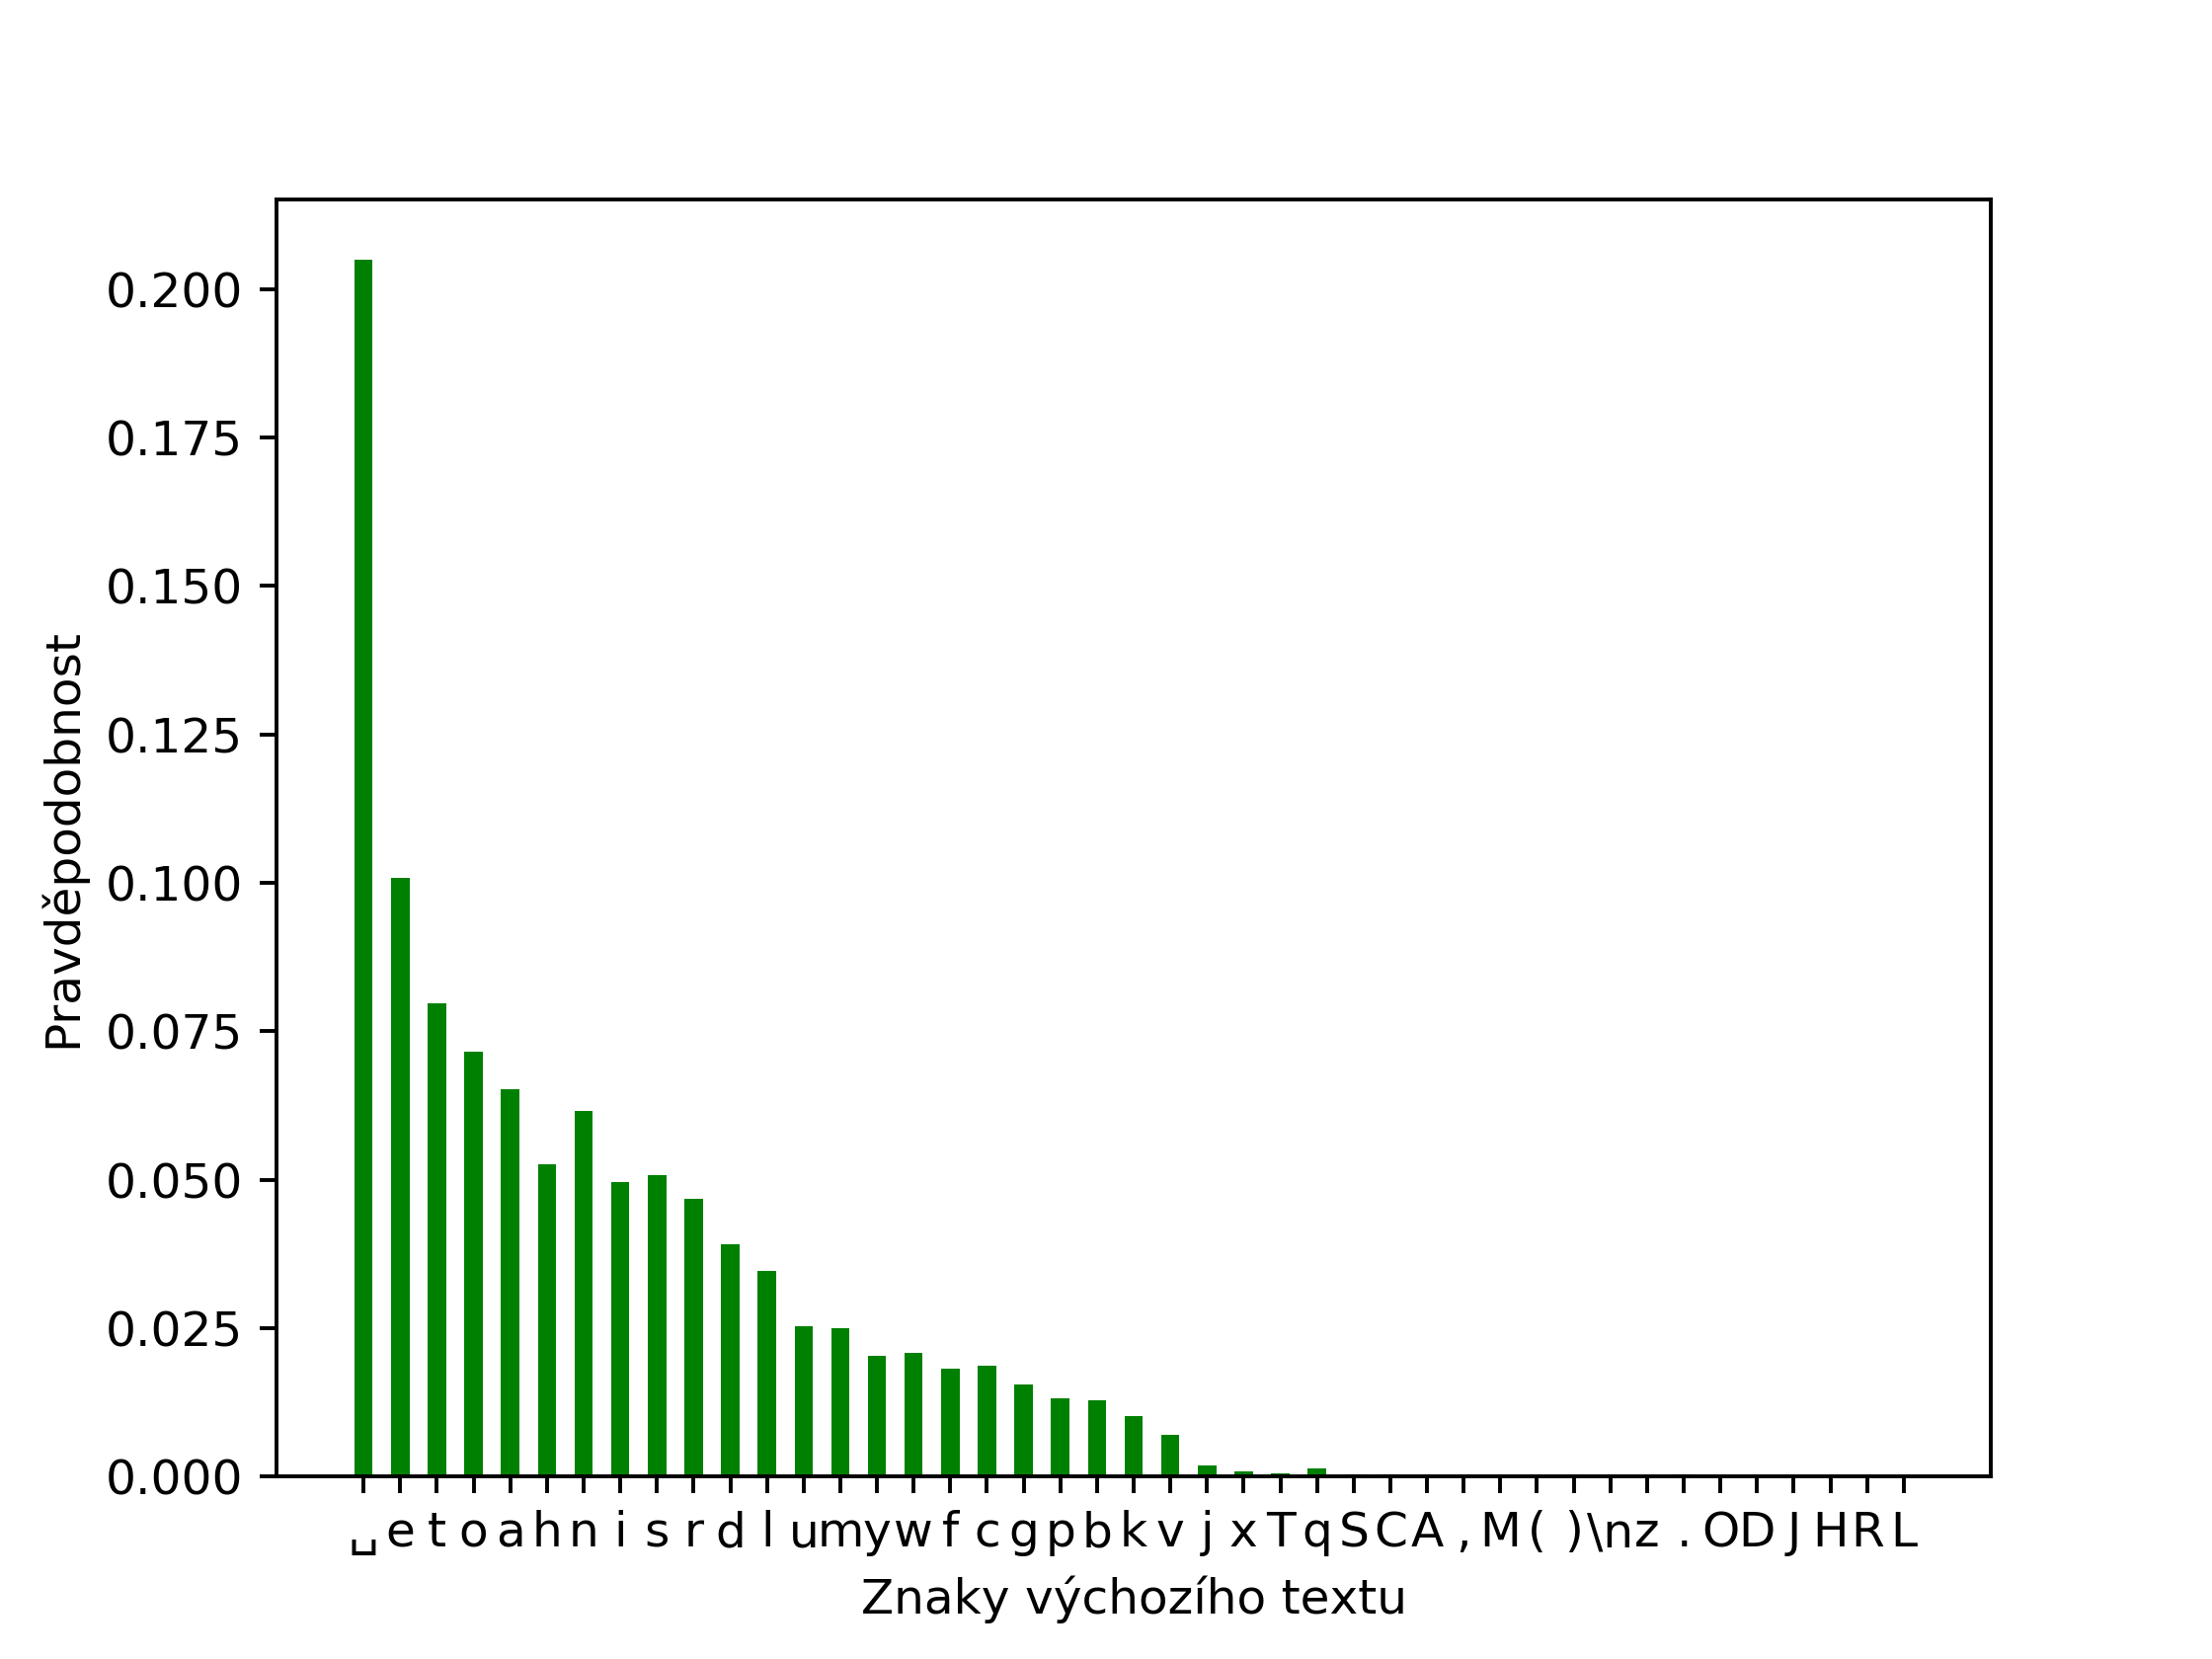
\includegraphics[scale=0.7]{../009_char_prob.png}\centering\caption{Graf závislosti velikosti instance na čase výpočtu.}\label{ZKC_graph}
\end{figure}

\begin{figure}[!htb]
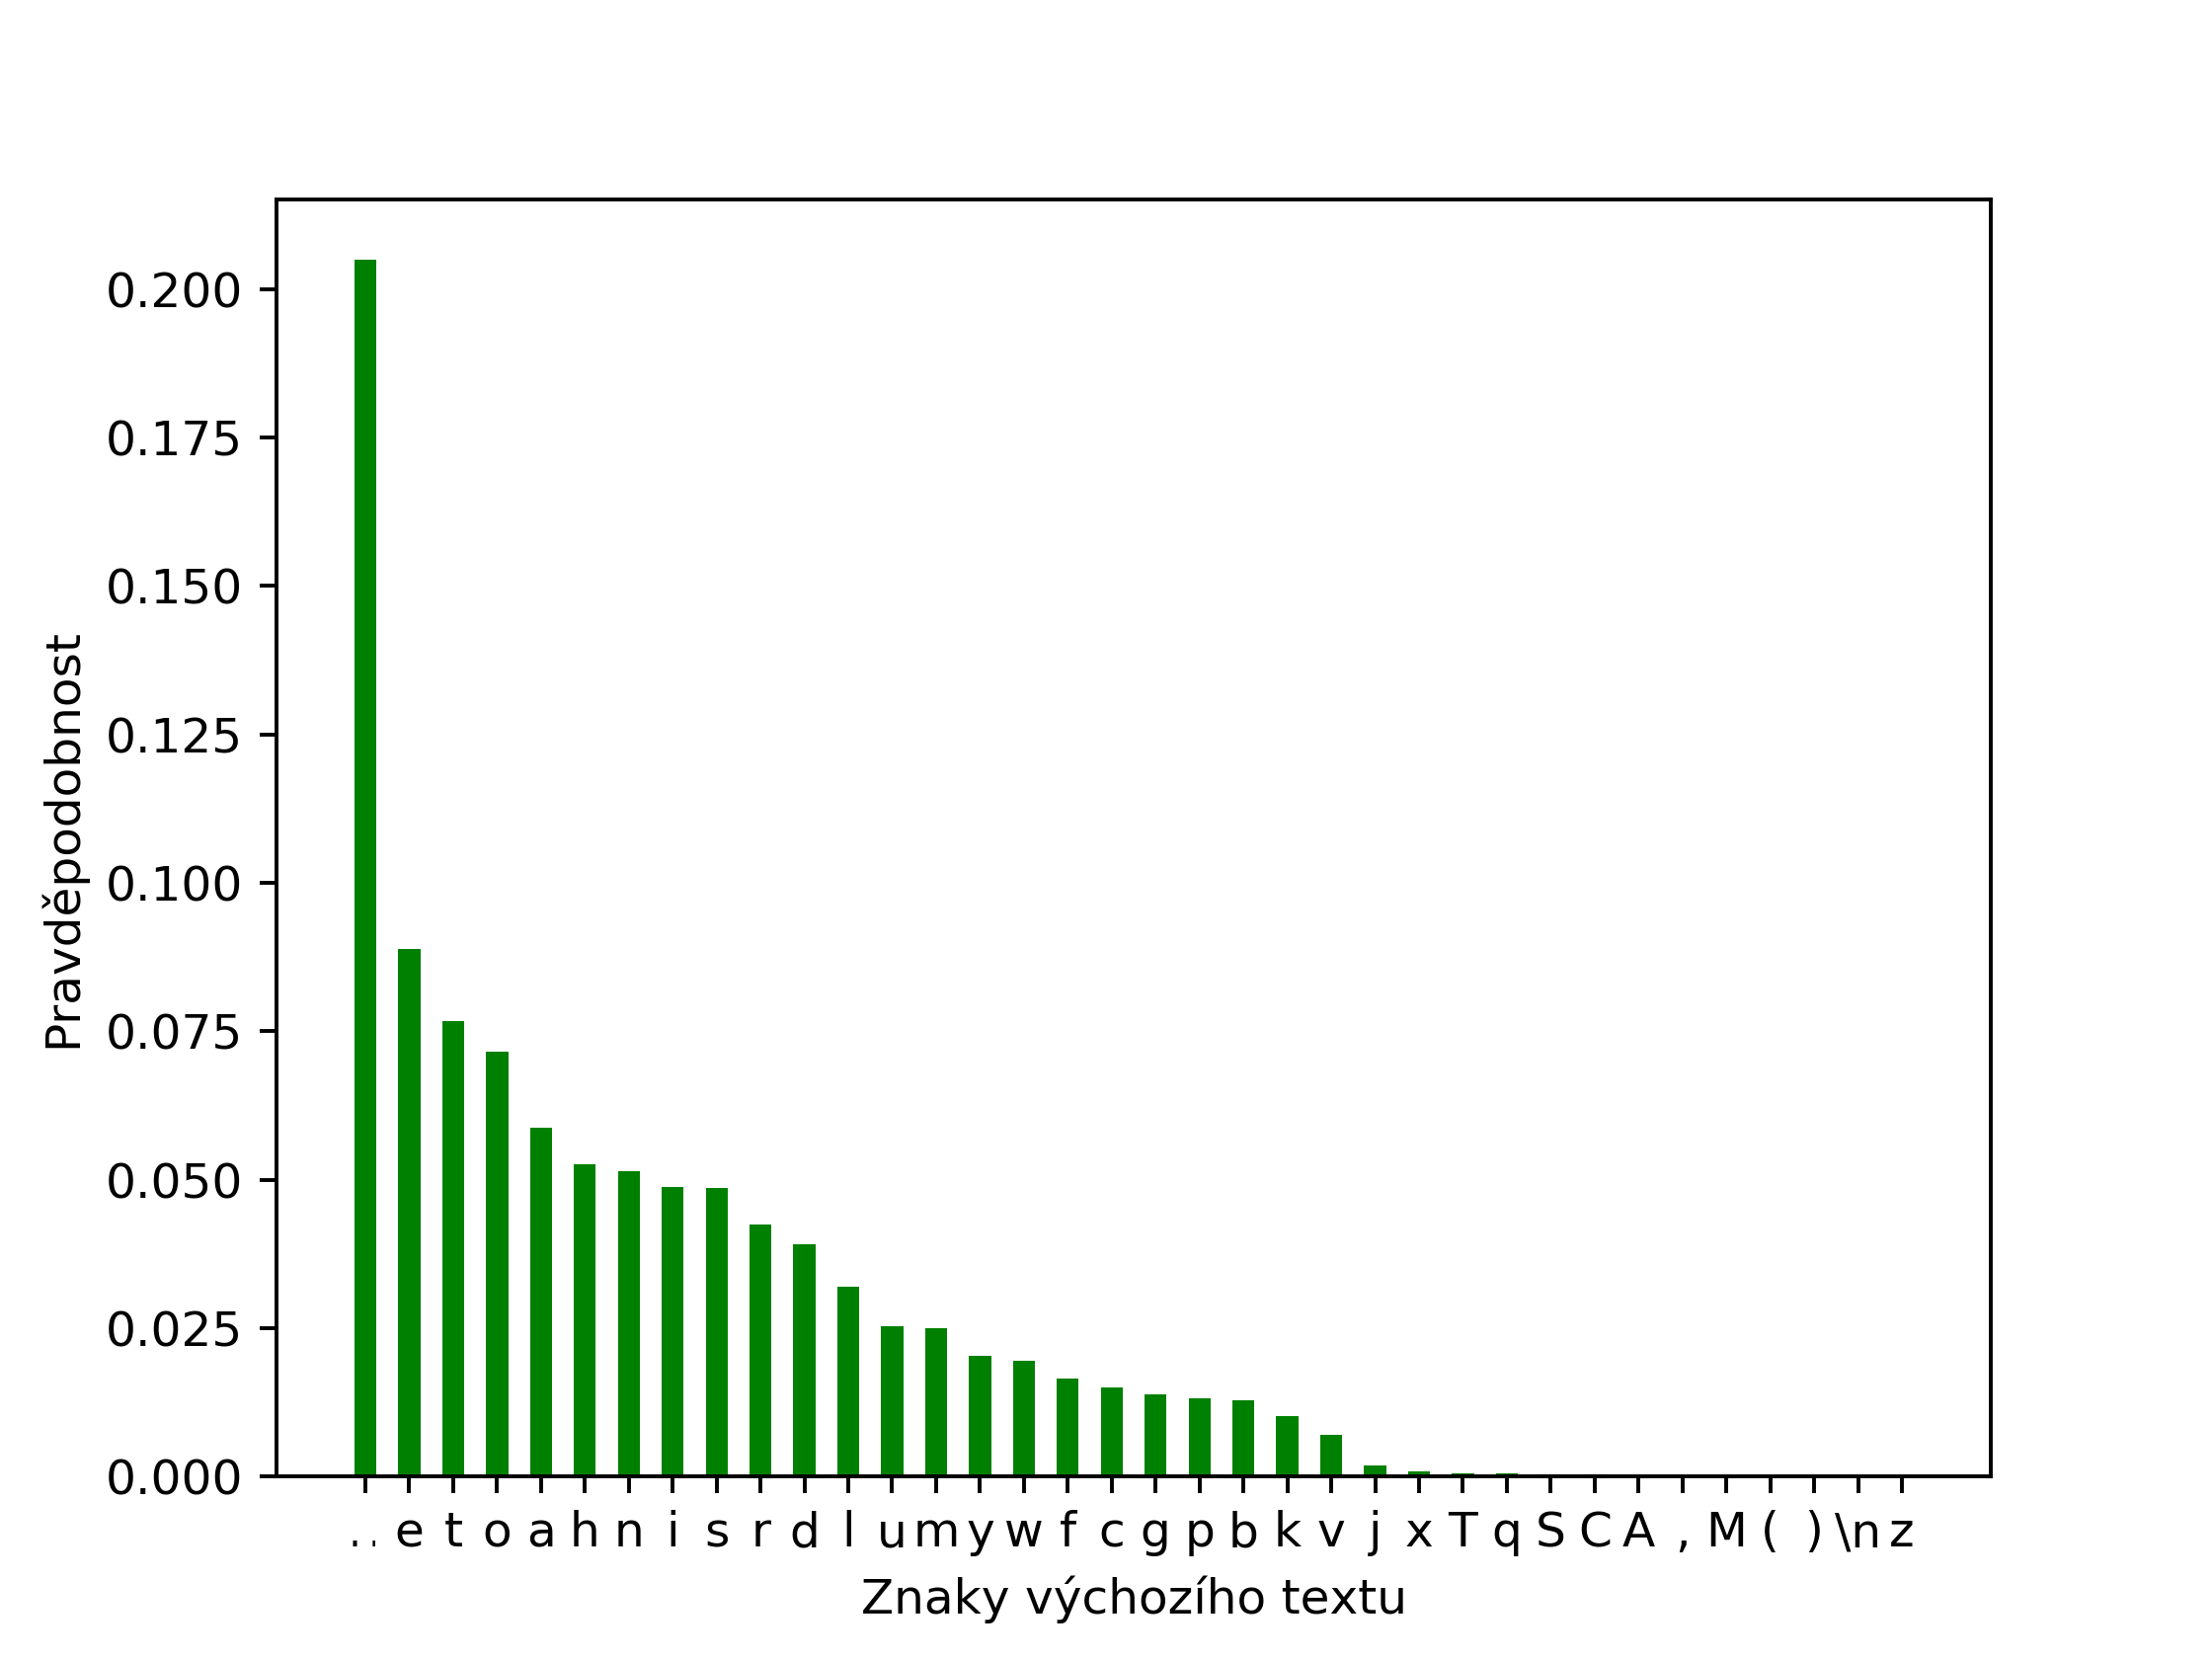
\includegraphics[scale=0.7]{../011_char_prob.png}\centering\caption{Graf závislosti velikosti instance na čase výpočtu.}\label{ZKW_graph}
\end{figure}

   	\section{Zhodnocení výsledků}
		Časová náročnost dynamického programování je způsobena převážně implementací algoritmu, který nejprve inicializuje všechny hodnoty tabulky a následně je všechny prochází. Tento postup je časově a paměťově náročný v závislosti na rostoucím součtu cen předmětů. Rychlost růstu složitosti tak odpovídá vzorci popsaném v sekci \ref{dp}.
		
		Náročnost FPTAS se dle předpokladu mění v závislosti na zadané přesnosti. Vyšší přesnost znamená větší časovou náročnost. Zároveň je z naměřených dat patrné, že se zvyšující se přesností snižuje maximální pozorovaná chyba. U náhodných dat jsou výsledky ovlivněny případy, kdy došlo aplikováním zjednodušení k výběru prázdného batohu jako nejlepšího řešení, i když bylo možné některý předmět do batohu vložit. V takovém případě je v datech patrná chyba $100\%$.
		
		Použité heuristiky byly pro všechny instance, dle předpokladu, časově nejméně náročné. Zároveň je pro ně pozorována největší chybovost pro všechny instance všech sad. Zajímavá je extrémně vysoká chybovost poměrové heuristiky u sady ZKW. Toto pozorování naznačuje, že byla data této sady volena jako příklad selhání této heuristiky. Pro volbu případu selhání poměrové heuristiky byl pravděpodobně volen jeden předmět s vysokou cenou který se po zařazení předmětů s lepším poměrem už nevejde, přestože by byl sám součástí optimálního řešení. Z tohoto důvodu vychází na této sadě heuristika uvažující jeden nejcennější předmět s výrazně menší chybou než u ostatních sad.
		
 
\end{document}